\scanpage{24}
\mspage{23}
\figure{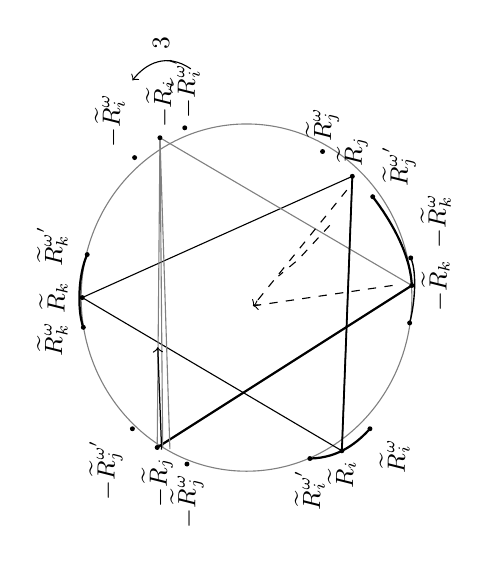
\begin{tikzpicture}[x=.7cm,y=.7cm,every node/.style={font=\small}]
\begin{scope}[rotate=90,transform shape]
\draw[gray] (0,0) ellipse (3.15 and 3.0);
\draw (0,2.98)--(-2.78,-1.73)--(2.2,-1.92)--cycle;
\draw[gray] (-2.72,1.62)--(2.9,1.57)--(.22,-3.0)--cycle;
\draw[line width=.8pt] (-2.72,1.62)--(.22,-3.0);
\draw[line width=.65pt] (-2.78,-1.73)--(2.2,-1.92);
\draw[gray,line width=.4pt] (-2.72,1.52)--(2.9,1.57);
\draw[gray,line width=.4pt] (-2.75,1.39)--(2.9,1.57);
\draw[->,line width=.45pt] (-2.76,1.54)--(-.9,1.61);
\draw[line width=.8pt] (-.54,2.96)..controls(-.25,3.07)and(.41,3.06)..(.78,2.89);
\draw[line width=.8pt] (-2.92,-1.15)..controls(-2.91,-1.7)and(-2.6,-2.04)..(-2.38,-2.24);
\draw[line width=.8pt] (1.83,-2.29)..controls(1.41,-2.61)and(.81,-2.97)..(.22,-3.0);
\draw[line width=.5pt] (-.46,-2.96)..controls(-.13,-3.05)and(.45,-3.1)..(.72,-2.98);
\draw[->,dashed] (.22,-2.65)--(-.15,-.12);
\draw[->,dashed] (1.95,-1.82)--(-.15,-.12);
\draw[dashed] (1.31,-1.51)--(.69,-.94)--(.39,-.58);
\foreach \p in {(-.54,2.96),(0,2.98),(.78,2.89),(-2.38,2.07),(-2.72,1.62),(-3.02,1.08),(-2.92,-1.15),(-2.78,-1.73),(-2.38,-2.24),(-.46,-2.96),(.22,-3.0),(.72,-2.98),(1.83,-2.29),(2.2,-1.92),(2.65,-1.38),(2.54,2.03),(2.9,1.57),(3.08,1.12)}{\fill \p circle(.045);}
\node[above] at (-.75,3.07) {$\widetilde R_k^\omega$};
\node[above] at (0,3.07) {$\widetilde R_k$};
\node[above] at (.94,3.07) {$\widetilde R_k^{\omega'}$};
\node[above left] at (-2.38,2.07) {$-\widetilde R_j^{\omega'}$};
\node[left] at (-2.72,1.62) {$-\widetilde R_j$};
\node[left] at (-3.02,1.08) {$-\widetilde R_j^\omega$};
\node[left] at (-2.92,-1.15) {$\widetilde R_i^{\omega'}$};
\node[left] at (-2.78,-1.73) {$\widetilde R_i$};
\node[below left] at (-2.38,-2.24) {$\widetilde R_i^\omega$};
\node[below] at (.22,-3.0) {$-\widetilde R_k$};
\node[below right] at (.72,-2.98) {$-\widetilde R_k^\omega$};
\node[below right] at (1.83,-2.29) {$\widetilde R_j^{\omega'}$};
\node[right] at (2.2,-1.92) {$\widetilde R_j$};
\node[right] at (2.65,-1.38) {$\widetilde R_j^\omega$};
\node[above right] at (2.54,2.03) {$-\widetilde R_i^\omega$};
\node[right] at (2.9,1.57) {$-\widetilde R_i$};
\node[right] at (3.08,1.12) {$\unsure{-}\widetilde R_i^{\unsure{\omega'}}$};
\draw[->] (4.15,1.01)..controls(4.45,1.45)and(4.25,1.83)..(3.94,2.07);
\node[right] at (4.32,1.55) {$3$};
\end{scope}
\end{tikzpicture}}

\figure{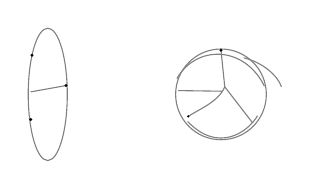
\begin{tikzpicture}[x=.8cm,y=.8cm]
\draw[gray] (0,0) ellipse (.31 and 1.05);
\draw[gray] (-.27,.04)--(.29,.14);
\fill (-.25,.62) circle(.025);\fill(-.27,-.4)circle(.025);\fill(.29,.14)circle(.025);
\begin{scope}[xshift=2.2cm]
\draw[gray] (0,0) circle(.72);
\draw[gray] (-.7,.25)..controls(-.4,.78)and(.36,.79)..(.69,.13);
\draw[gray](-.53,-.43)..controls(-.03,-.95)and(.44,-.58)..(.58,-.34);
\draw[gray](0,.7)--(.06,.12)--(.5,-.45);
\draw[gray](.06,.12)..controls(-.04,-.12)and(-.34,-.23)..(-.52,-.35);
\draw[gray](-.68,.06)--(.02,.05);
\draw[gray](.36,.58)..controls(.66,.51)and(.9,.3)..(.96,.12);
\fill (0,.7)circle(.025);\fill(-.52,-.35)circle(.02);
\end{scope}
\end{tikzpicture}}

\figure{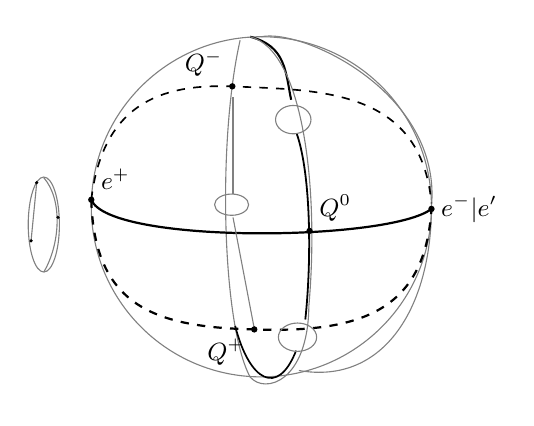
\begin{tikzpicture}[x=.9cm,y=.9cm,every node/.style={font=\small}]
\draw[gray] (0,0) circle(2.4);
\draw[gray] (0,2.4)..controls(.58,2.52)and(2.55,1.61)..(2.4,0)..controls(2.4,-1.4)and(1.74,-2.52)..(.53,-2.31);
\draw[gray](-.3,2.35)..controls(-.62,.95)and(-.56,-1.65)..(-.16,-2.4);
\draw[line width=.75pt](-.16,2.4)..controls(.35,2.27)and(.34,1.9)..(.42,1.51);
\draw[line width=.65pt](.5,1.03)..controls(.7,.45)and(.71,-.75)..(.62,-1.59);
\draw[line width=.6pt](.49,-2.03)..controls(.23,-2.69)and(-.17,-2.46)..(-.37,-1.68);
\draw[gray](-.16,2.4)..controls(.58,2.22)and(.82,.3)..(.67,-1.4)..controls(.66,-2.47)and(.05,-2.65)..(-.16,-2.4);
\draw[dashed,line width=.6pt](-2.4,.1)..controls(-2.23,1.54)and(-1.3,1.73)..(-.41,1.7)..controls(.76,1.64)and(2.25,1.7)..(2.4,.05);
\draw[line width=.8pt](-2.4,.1)..controls(-2.15,-.53)and(1.8,-.49)..(2.4,-.03);
\draw[dashed,line width=.8pt](-2.4,.1)..controls(-2.36,-1.41)and(-1.49,-1.7)..(-.1,-1.73)..controls(1.37,-1.78)and(2.31,-1.49)..(2.4,-.03);
\draw[gray](-.42,.03)ellipse(.24 and .15);
\draw[gray](.45,1.23)ellipse(.25 and .2);
\draw[gray](.51,-1.84)ellipse(.27 and .2);
\draw[gray](-.4,.18)--(-.4,1.55);
\draw[gray](-.4,-.15)--(-.1,-1.72);
\foreach \p in {(-2.4,.1),(2.4,-.03),(.68,-.34),(-.41,1.7),(-.1,-1.73)}{\fill\p circle(.045);}
\node[above right]at(-2.4,.1){$e^+$};
\node[right]at(2.4,-.03){$\unsure{e^-|e'}$};
\node[above right]at(.68,-.34){$\unsure{Q}^0$};
\node[above left]at(-.41,1.7){$\unsure{Q}^-$};
\node[below left]at(-.1,-1.73){$\unsure{Q}^{\unsure{+}}$};
\draw[gray](-3.07,-.25)ellipse(.22 and .67);
\draw[gray](-3.07,.41)..controls(-2.8,.1)and(-2.84,-.53)..(-3.07,-.92);
\draw[gray](-3.25,-.48)--(-3.17,.34);
\fill(-3.17,.34)circle(.025);\fill(-3.25,-.48)circle(.025);\fill(-2.87,-.15)circle(.025);
\end{tikzpicture}}

\figure{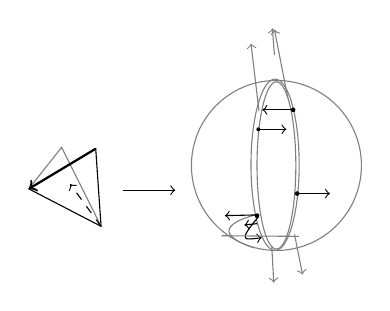
\begin{tikzpicture}[x=.85cm,y=.85cm]
\draw (-3.1,.1)--(-2.1,.7)--(-2.02,-.46)--cycle;
\draw[gray](-3.1,.1)--(-2.61,.72)--(-2.02,-.46);
\draw[->,line width=.8pt](-2.1,.7)--(-3.1,.1);
\draw[->,dashed](-2.02,-.46)--(-2.48,.17);
\draw[->](-1.69,.08)--(-.91,.08);
\draw[gray](.6,.45)circle(1.27);
\draw[gray](.6,.45)ellipse(.29 and 1.25);
\draw[gray](.58,.46)ellipse(.36 and 1.28);
\draw[->](.31,-.42)--(.12,-.44);
\draw[->](.91,.03)--(1.4,.03);
\draw[->](.85,1.28)--(.39,1.28);
\draw[->](.33,.99)--(.75,.99);
\draw[->,gray](.53,-.75)--(.56,-1.3);
\draw[->,gray](.87,-.58)--(.99,-1.18);
\draw[->,gray](.34,1.26)--(.22,2.27);
\draw[->,gray](.77,1.46)--(.57,2.48);
\draw[->,gray](.57,2.1)--(.54,2.5);
\draw[gray](.28,-.29)..controls(-.23,-.43)and(-.24,-.61)..(.26,-.78);
\draw[->](.28,-.29)--(-.17,-.3);
\draw[->](.33,-.32)..controls(.01,-.7)and(.12,-.66)..(.38,-.63);
\draw[gray](-.22,-.6)--(.94,-.61);
\fill(.31,-.3)circle(.035);\fill(.91,.03)circle(.035);\fill(.85,1.28)circle(.035);\fill(.33,.99)circle(.03);
\end{tikzpicture}}
